%structure taken from the fischsheet https://bitbucket.org/toman/fischsheet

%template by http://stdout.org/~winston/latex/

\documentclass[10pt,landscape,a4paper]{article}
\usepackage{multicol}
\usepackage{calc}
\usepackage{ifthen}
\usepackage[landscape]{geometry}
\usepackage{amsmath,amsthm,amsfonts,amssymb}
\usepackage{color,graphicx,overpic}
\usepackage{hyperref}
\usepackage{txfonts}
\usepackage[latin1]{inputenc}
\usepackage[T1]{fontenc}
\usepackage[ngerman]{babel}
\usepackage{listings}
\usepackage{pdfpages}
\lstset{tabsize = 3}


\pdfinfo{
  /Title (Cheatsheet #define true false)
  /Creator (TeX)
  /Author (Lukas, Quirin, Sebastian)
  /Subject (Cheatsheet for NWERC 2014)
}

% This sets page margins to .5 inch if using letter paper, and to 1cm
% if using A4 paper. (This probably isn't strictly necessary.)
% If using another size paper, use default 1cm margins.
\geometry{top=.45in,left=.5in,right=.5in,bottom=.5in}

% Turn off header and footer
\pagestyle{empty}

% Redefine section commands to use less space
\makeatletter
\renewcommand{\section}{\@startsection{section}{1}{0mm}%
                                {-1ex plus -.5ex minus -.2ex}%
                                {0.5ex plus .2ex}%x
                                {\normalfont\large\bfseries}}
\renewcommand{\subsection}{\@startsection{subsection}{2}{0mm}%
                                {-1explus -.5ex minus -.2ex}%
                                {0.5ex plus .2ex}%
                                {\normalfont\normalsize\bfseries}}
\renewcommand{\subsubsection}{\@startsection{subsubsection}{3}{0mm}%
                                {-1ex plus -.5ex minus -.2ex}%
                                {1ex plus .2ex}%
                                {\normalfont\small\bfseries}}
\makeatother

% Define BibTeX command
\def\BibTeX{{\rm B\kern-.05em{\sc i\kern-.025em b}\kern-.08em
    T\kern-.1667em\lower.7ex\hbox{E}\kern-.125emX}}

% Don't print section numbers
\setcounter{secnumdepth}{0}


\setlength{\parindent}{0pt}
\setlength{\parskip}{0pt plus 0.5ex}

%My Environments
\newtheorem{example}[section]{Example}
% -----------------------------------------------------------------------

\usepackage{fancyhdr}
\pagestyle{fancy}
\setlength{\headheight}{17pt} 
\lhead{Technische Universit\"at M\"unchen}
\rhead{\thepage}
\fancyfoot{}

\begin{document}
\raggedright
\footnotesize
\begin{multicols}{2}


% multicol parameters
% These lengths are set only within the two main columns
%\setlength{\columnseprule}{0.25pt}
\setlength{\premulticols}{1pt}
\setlength{\postmulticols}{1pt}
\setlength{\multicolsep}{1pt}
\setlength{\columnsep}{2pt}

\begin{center}
     \Large{
     	Team Reference Document\\
     	\underline{Team \#define true false, TU M\"unchen}\\
     	NWERC 2014} \\
\end{center}

\tableofcontents


%\section{Graph algorithms}
%\input{shortest_path}

% You can even have references
%\rule{0.3\linewidth}{0.25pt}
\scriptsize
%\bibliographystyle{abstract}
%\bibliography{refFile}
\end{multicols}
\newpage
\addcontentsline{toc}{section}{Theoretical CS Cheat Sheet}
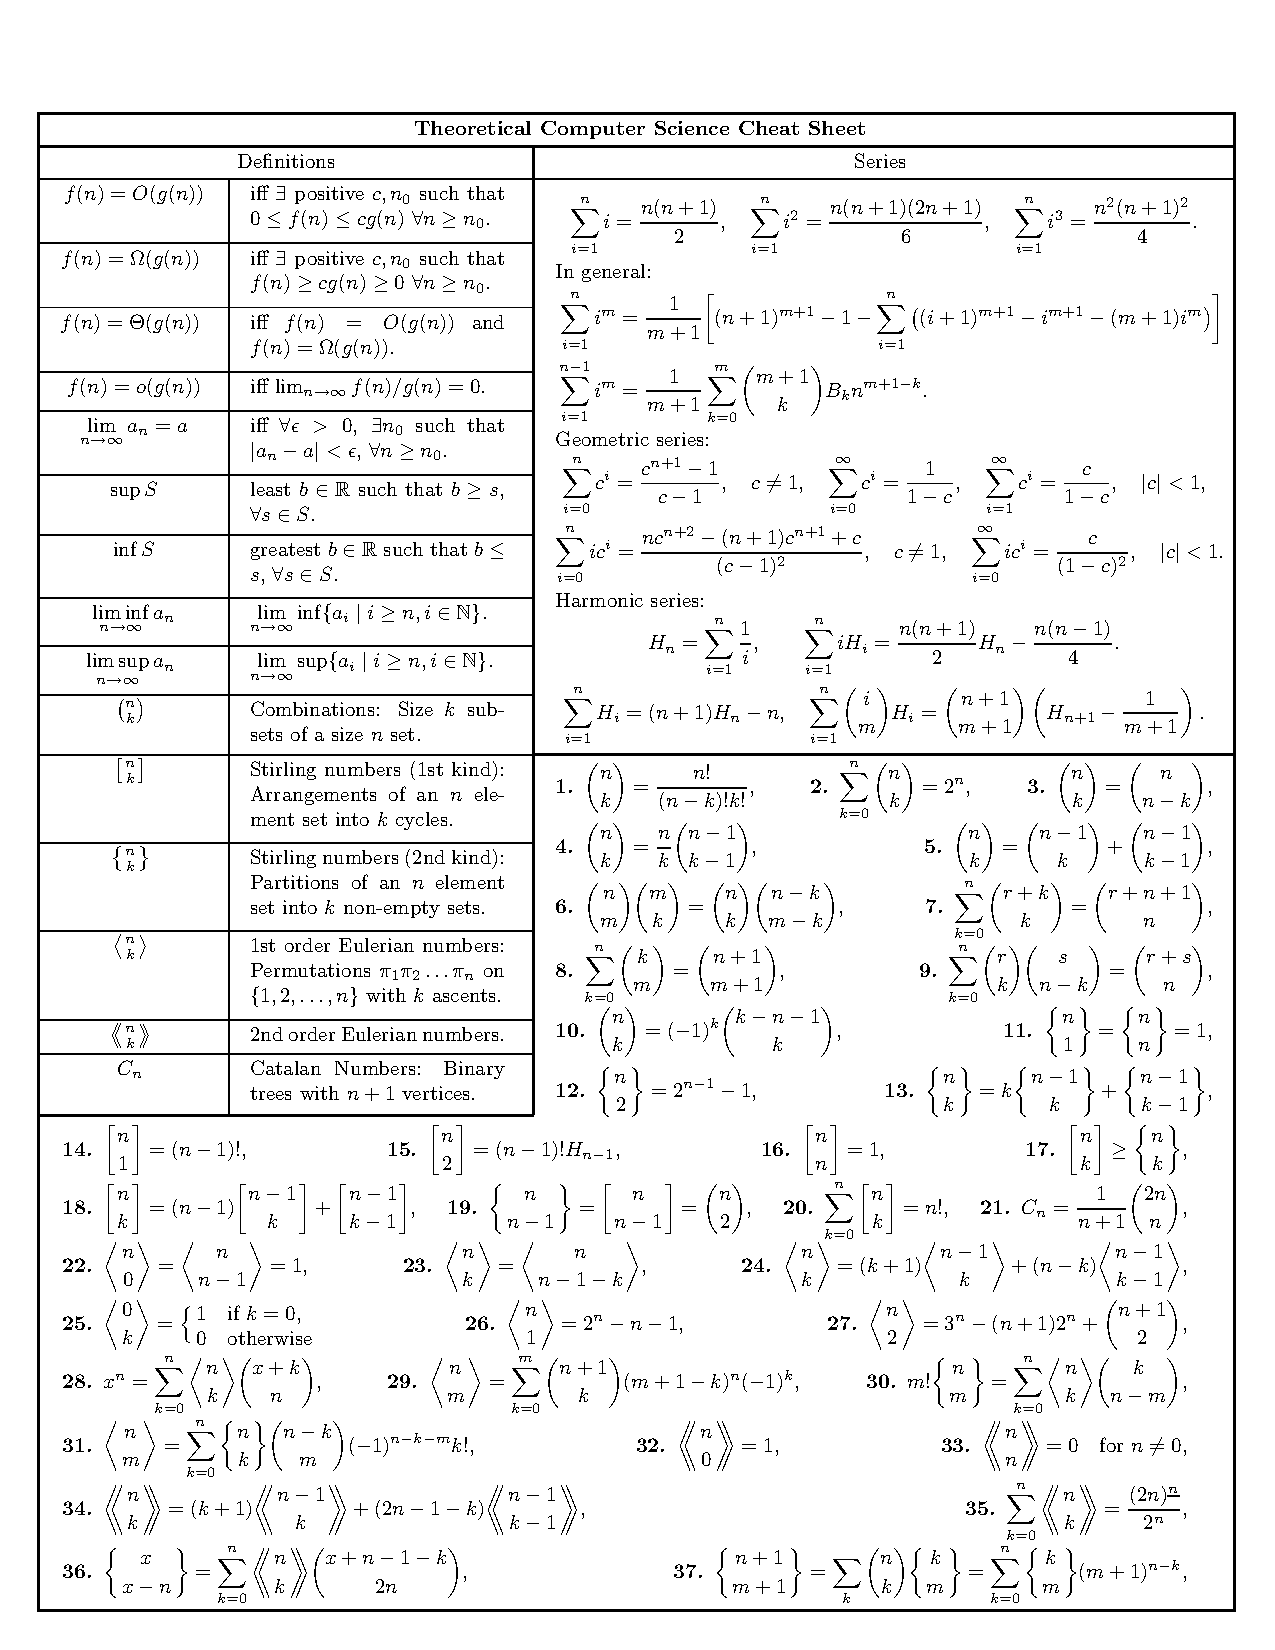
\includepdf[landscape=true,pages={1-5},pagecommand={\thispagestyle{fancy}}]{cheat}

\end{document}